\section{Experiment}
In this section, we describe our implementation of a real-time speaker diarization based on the proposed method.

\subsection{Implementation}
\begin{figure}[htb]
    \begin{minipage}[b]{1.0\linewidth}
    \centering
    \centerline{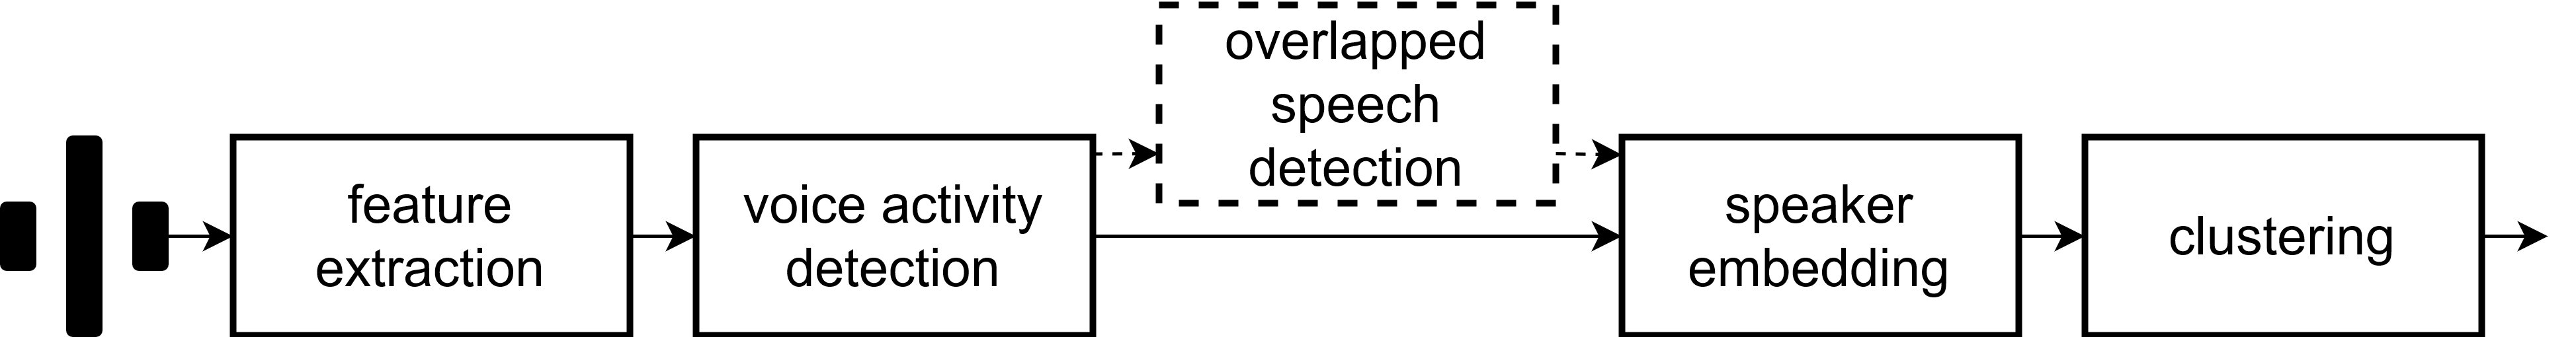
\includegraphics[width=8.5cm]{assets/speaker_diarization.png}}
    %\vspace{2.0cm}
    \end{minipage}
\caption{Speaker Diarization Pipeline}
\label{fig:speaker_diarization}
\end{figure}

Our speaker diarization pipeline, as illustrated in Figure \ref{fig:speaker_diarization}, consists of a feature extraction module converting audio waveform into spectrogram for each frame of 25ms length and 10ms shift. Then voice activity detection (VAD) is applied to isolate the non-speech segments. In this experiment, we adopt Silero VAD \cite{SileroVAD}, a large-scale model-based VAD engine available for public use. Next, the speech segments are passed through a universal background speaker ID model to get its 192-dimensional embedding feature representations, each for 0.96s segments, without overlap. We trained our own background model using ECAPA-TDNN architecture \cite{dawalatabad21_interspeech} using our own data consisting of more than 6000 thousand speakers, each having around 30 minutes of speech data.  Finally, the speech sequence of embedding features goes through a clustering module to get the speaker indices.  There was an overlapping speech detection module which is trained on an augmented speaker ID data, to provide extra overlapping detection timing, but it was turned off as we focus on comparing clustering methods.

\subsection{Reference Methods}
We test our proposed algorithm, which uses Frequent Direction with Block Krylov Iteration (SSC BKI) to construct the low-dimensional embedding of the stream. Three other algorithms are chosen for comparison: offline Spectral Clustering (SC) \cite{ng2001spectral}, Streaming Spectral Clustering (SSC) \cite{yoo2016streaming} and Online K-means (OKM) \cite{NIPS2011_52c67099}.

\subsection{Experiment Setup}

We conducted our experiments on files picked from two free public datasets: (1) IMDA3 \cite{koh19_interspeech} and (2) AMI Meeting Corpus \cite{carletta2005ami}, all summarized in Table \ref{tab:data}.

\begin{center}
\captionof{table}{Statistics of the experimental datasets}
\label{tab:data}
\begin{tabular}{| c | c | c | c |}
    \hline
    Dataset & \#instances & \#features & \#clusters\\
    \hline
    IMDA3 & 18 & 192 & 2\\
    \hline
    AMI test & 24 & 192 & 3, 4\\
    \hline
\end{tabular}
\end{center}

To show the stability of algorithms, we performed each $40$ times. As the number of speakers are much smaller than the embedding dimension, the number of singular vectors $k$ can be set empirically, according to practical situations. For example, in our experiment, the rooms are small hence we set $k = 8$. The actual number of speakers is then determined by the later online \textit{K-means} step. The size of sketch matrix is set to be $l = 14$ to contain enough information. The number of cosets in online \textit{K-means} is set to be $k \log n$ where $n$ is number of data points. 

\begin{comment}
    The number of clusters $k$ is determined by the "oracle" number of speakers. We set the picking batch size to be $64$, the size of the sketch matrix to be $l = 14$, where $m = 192$ is the dimension of speaker embedding, and the number of cosets in online \textit{K-means} to be $k \log n$ where $n$ is the number of data points.
\end{comment}

\subsection{Results and Performance Comparison}

\begin{center}
\captionof{table}{DER(\%) performance of the compared algorithms on IMDA3 and AMI dataset}
\label{tab:result}
\begin{tabular}{| c | c | c | c |}
    \hline
    Method & IMDA3 & AMI test \\
    \hline
    SC & $20.7$ & $24.4$ \\
    \hline
    OKM & $28.0$ & $33.3$ \\
    \hline
    SSC & $20.8$ & $26.1$ \\
    \hline
    SSC\_BKI & $\mathbf{20.7}$ & $\mathbf{25.2}$ \\
    \hline
\end{tabular}
\end{center}

Table \ref{tab:result} shows the general performance of the compared algorithms. For each dataset, we report the average \textit{Diarization Error Rate} (DER). We can make the following observations from these results:
\begin{enumerate}
    \item Online \textit{K-means} performance is far behind the standard offline \textit{Spectral Clustering} (SC) algorithm.
    \item With a compression rate of just around $7\%$, streaming methods (SSC, SSC-BKI) achieved almost similar results to the standard offline version.
    \item Compared with re-computation by offline \textit{Spectral Clustering}, it achieves similar accuracy but with much lower computational cost.
    \item With the adoption of \textit{Block Krylov Iteration}, SVD calculation is more robust and accurate, resulting in a slight improvement of DERs.
    \item \textit{Block Krylov Iteration} provides faster speed in the implementation, but this needs more comprehensive analysis.
\end{enumerate}





\begin{comment}
In this section, we experimentally test our proposed approach in terms of effectiveness and efficiency on speaker diarization task. Our speaker diarization pipeline consists of feature extraction, voice activate detection (\textit{Silero VAD}) \cite{SileroVAD}, segmentation, speaker embedding module (\textit{ECAPA-TDNN}) \cite{dawalatabad21_interspeech}, and streaming spectral clustering algorithm as shown in Figure \ref{fig:speaker_diarization}.



\subsection{Implementation}

\subsection{Reference Methods}


\subsection{Experiment Setup}
\textbf{Dataset} We conducted our experiments on two free public datasets: (1) IMDA3 \cite{koh19_interspeech} and (2) AMI Meeting Corpus \cite{7529878bc1a143dbad4fa019e742fdb8}, all summarized in Table \ref{tab:data}.

\textbf{Algorithm} We test our proposed algorithm, which uses Frequent Direction with Block Krylov Iteration (SSC\_BKI) to construct
the low-dimensional embedding of the stream. Three other algorithms are chosen for comparison: offline \textit{Spectral Clustering} (SC) \cite{ng2001spectral},\textit{ Streaming Spectral Clustering} (SSC) \cite{yoo2016streaming} and \textit{Online K-means} (OKM) \cite{NIPS2011_52c67099}.

\textbf{Evaluation Metrics and Parameter Settings} To show the stability of each algorithm, we performed the each algorithm $40$ times. The number of clusters $k$ in the datasets is assumed to be known a priori. We set the picking batch size to be $64$, size of the sketch matrix to be $14 \approx \sqrt{d}$ where $d = 192$ is the dimension of speaker embedding, the number of cosets in streaming K-means to be $k \log n$ where $k$ is the number of data points.

\subsection{Results and Performance Comparison}

Table \ref{tab:result} shows the general performance of the compared algorithms. For each dataset, we report the average Diarization Error Rate (DER). We can make the following observations from
these results:
\begin{enumerate}
    \item Even though the \textit{ECAPA-TDNN} embeddings from the datasets are not low-rank, picking the size of sketch matrix to be $\sqrt{d}$ nearly recover the performance of offline algorithm.
    \item DERs of \textit{SSC} and \textit{SSC\_BKI} are much more stable across different datasets despite using the same underlying \textit{Stream K-means} algorithm.
    \item Compared with re-computation by offline \textit{Spectral Clustering}, it achieves similar accuracy but with much lower computational cost. 
\end{enumerate}



\end{comment}